\section{Proposed Solution}
\label{sec:method}

Recently some vision foundation models such as DINOv2~\cite{oquab2023dinov2} have emerged and demonstrated robust performance across a range of downstream tasks. Indeed many top-performing solutions in open challenges are built upon fine-tuning large vision models. However, since the competition only allows to use ImageNet-1K pretrained backbones, we turn our focus to the problem nature of the task and mainly address the challenges we observe above.
The overview of our solution is % visualized
shown in Fig.~\ref{fig:pipeline}. Our solution includes three stages: training a supervised segmentation baseline, applying a semi-supervised semantic segmentation pipeline, and leveraging a sliding-window-style test-time scaling strategy. % Recently, many robust vision foundation models, such as DINOv2, have emerged and significantly improved performance across a wide range of downstream tasks. In fact, many top-performing solutions in open challenges are built upon fine-tuning large vision models. However, this competition restricts the use of pretrained models to those trained only on ImageNet-1k. As a result, we return our focus to the core of the task and address the challenges we have observed step by step.

% Our baseline is based on Mask2Former architecture. Since the ViT-Adapter backbone shows certain advantages in dense prediction tasks, we also replaced the standard SwinTransformer backbone with ViT-Adapter.

% There are two stages in our training process. In the first stage, we train our refined model on the entire training dataset. In the second stage, we adopt a guided distillation pipeline~\cite{} to train a robust model using both labeled data and selected unlabeled data.

\subsection{SAPA-Enhanced ViT-Adapter}

We choose the ViT-Adapter~\cite{chen2022vision} as our baseline, because current state-of-the-art semantic segmentation models are typically based on the architecture of vision transformer (ViT)~\cite{dosovitskiy2021image}. In particular, we adopt the BEiTv2 and ImageNet-1K pretrained ViT-Large model.\footnote{\url{https://github.com/microsoft/unilm/blob/master/beit2/get_started_for_image_classification.md}} 
By feeding the input image tokens into the ViT-Adapter, multi-scale features $\{\mathcal{F}_1^{\frac{1}{4}},\mathcal{F}_2^{\frac{1}{8}},\mathcal{F}_3^{\frac{1}{16}},\mathcal{F}_4^{\frac{1}{32}} \}$ are extracted, followed by the Mask2Former head~\cite{he2022masked}. In the pixel decoder of Mask2Former, the three low-resolution features $\{\mathcal{F}_2^{\frac{1}{8}},\mathcal{F}_3^{\frac{1}{16}},\mathcal{F}_4^{\frac{1}{32}}\}$ are refined through several layers of multi-scale deformable attention~\cite{xia2022vision}, and the output are denoted by \{$\mathcal{O}_2^\frac{1}{8}$, $\mathcal{O}_3^\frac{1}{16}$, $\mathcal{O}_4^\frac{1}{32}$\}. The decoder feature $\mathcal{O}_2^{\frac{1}{8}}$ is upsampled and fused with $\mathcal{F}_1^{\frac{1}{4}}$ to obtain the mask feature $\mathcal{F}_{\text{mask}}$, and $\mathcal{F}_{\text{mask}}$ is jointly used with the mask query embedding $\mathcal{Q}_{mask}$ to predict final segmentation mask $M$ as
\begin{equation}\label{eq:mask}
    M=g(\mathcal{Q}_{mask},\mathcal{F}_{mask})\,,
\end{equation}
where $g(\cdot)$ is the mask predictor.
Eq.~\eqref{eq:mask} indicates that the quality of $\mathcal{F}_{\text{mask}}$ is % strongly correlated
closely related to % with 
the quality of the final predicted masks $M$.

Recall that our goal is to enhance the prediction of the \texttt{stem} class. The fine structure of the stem requires the model to have clear detail delineation in the high-resolution mask feature $\mathcal{F}_{\text{mask}}$. According to open literature~\cite{lu2019indices,lu2022index,lu2022fade,lu2022sapa,liu2023learning,lu2025fade}, one critical stage that affects the quality of $\mathcal{F}_{\text{mask}}$ is feature upsampling. Unfortunately, the standard Mask2Former head uses bilinear interpolation for upsampling, which would \textit{ipso facto} blur details. Hence, we propose to replace bilinear upsampling with SAPA~\cite{lu2022sapa} to enhance the detail awareness of the model.
% To enhance the model's understanding of fine details, we incorporate the SAPA~\cite{lu2022sapa} upsampling operator into the pixel decoder of Mask2Former.  In the pixel decoder of Mask2Former, the  The decoder feature $\mathcal{O}_2^{\frac{1}{8}}$ is upsampled and fused with $\mathcal{F}_1^{\frac{1}{4}}$ to obatin the mask feature. And the mask feature is jointly used with the query embeddings to generate the predicted masks. Thus, the quality of the mask features is strongly correlated with the quality of the final predicted masks. So we replace the default bilinear interpolation upsampling with the SAPA-G upsampling operator. 

\begin{table}[!t]
    \renewcommand{\arraystretch}{1.5}
    \addtolength{\tabcolsep}{-1pt}
    \centering
    \begin{tabular}{@{}lcccc@{}}
    \toprule
        \multirow{2}*{\textbf{data splits}} & \multicolumn{2}{c}{\textbf{training}} & \multirow{2}*{\textbf{validation}} & \multirow{2}*{\textbf{testing}} \\
    \cline{2-3}
        & \textbf{labeled} & \textbf{unlabeled} & & \\
    \hline
        \#Images & $99$ & $64,368$ & $99$ & $110$   \\
    \bottomrule
    \end{tabular}
    \caption{\textbf{Training, validation, the testing splits of the GWFSS competition dataset}.}
    \label{tab:dataset_data_num}
\end{table}

% \FloatBarrier
\begin{figure*}[!t]
    \centering
    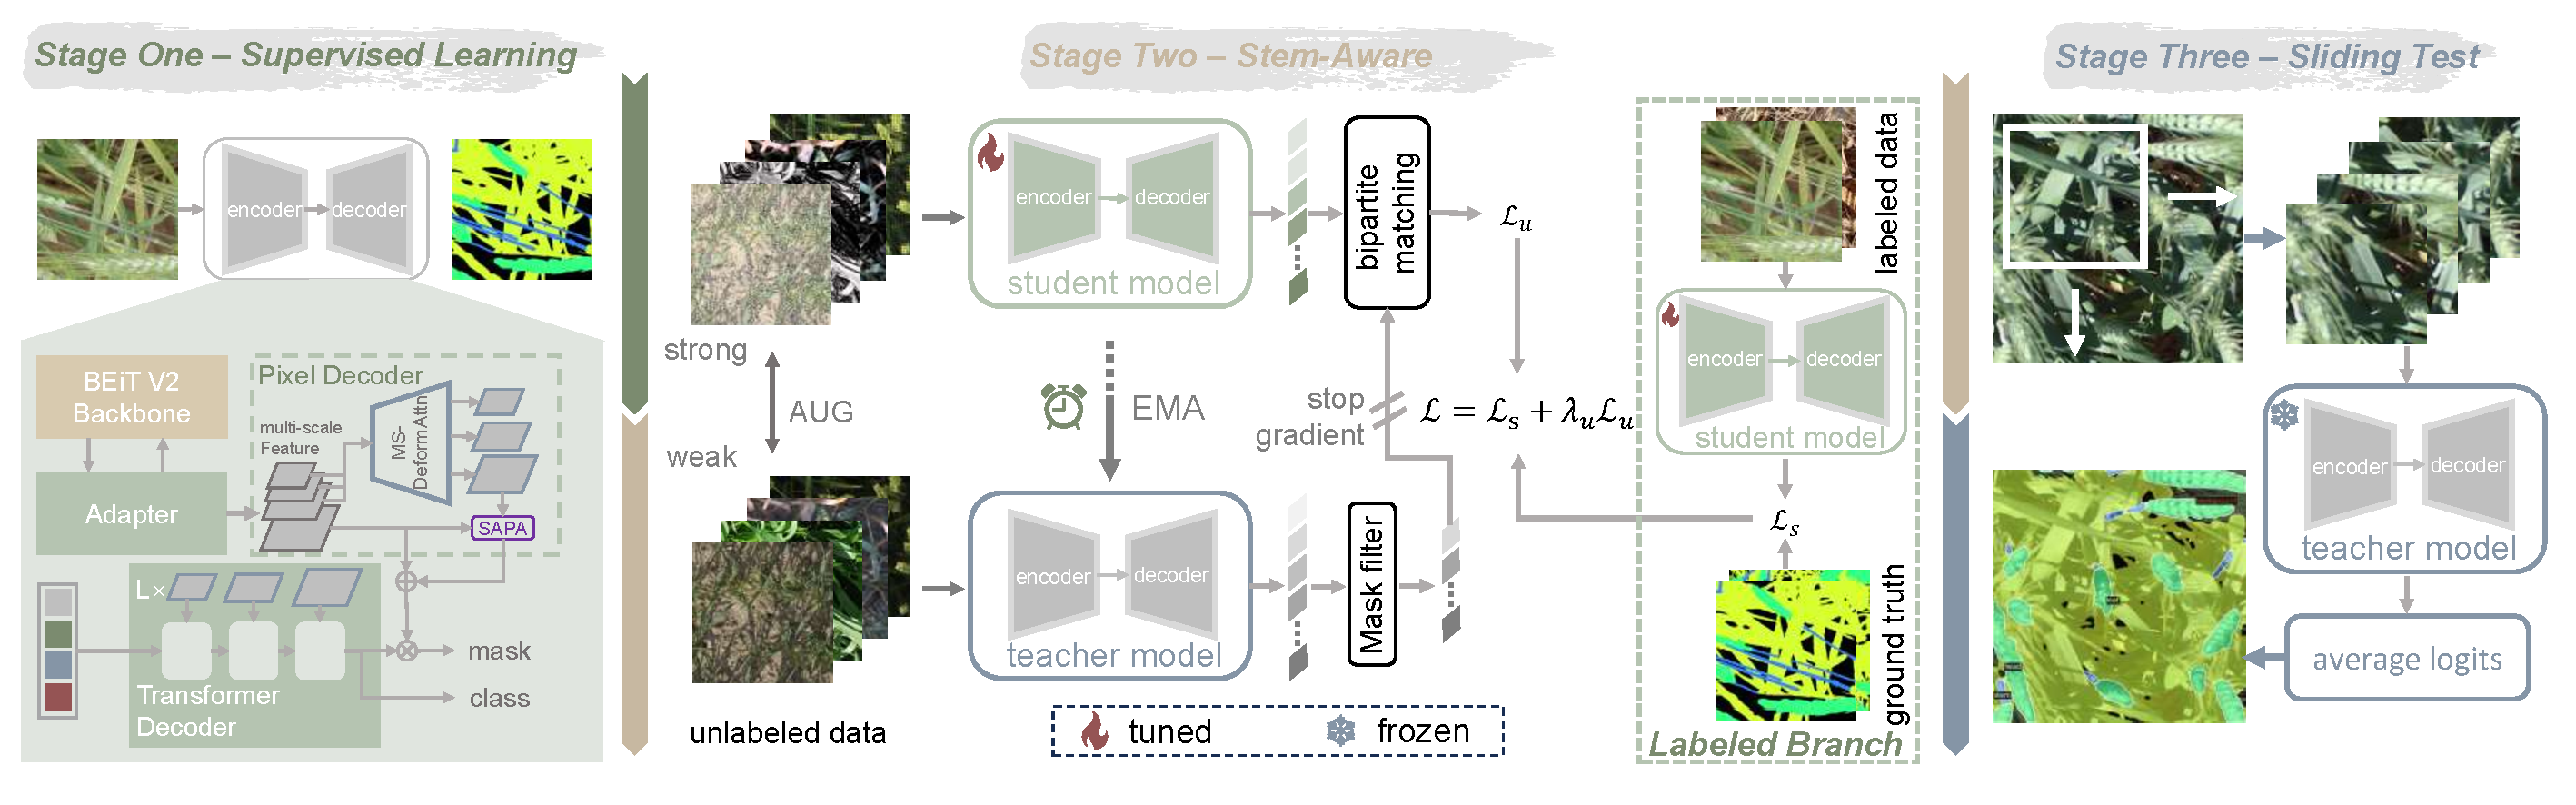
\includegraphics[width=\linewidth]{pipeline.pdf}
    \caption{\textbf{The overview of our solution}. Our solution includes three stages: in stage one, we leverage the labeled training dataset to train a supervised baseline ViT-Adapter and enhance its detail delineation with a dynamic upsampler SAPA; in stage two, we apply a semi-supervised learning pipeline with guided distillation on both labeled data and selected unlabeled data; in stage three, we implement a form of test-time scaling by zooming in images and segmenting twice following the sliding-window-style inference. }
    \label{fig:pipeline}
\end{figure*}
% \FloatBarrier

SAPA % considers 
enhances detail delineation by modeling the mutual similarity between % correlated points
the low-resolution decoder neighborhood and the high-resolution encoder feature point in the upsampling kernel. % enabling the upsampled feature maps to preserve edges while avoiding the introduction of excessive noise. Specifically
Formally, given a local decoder neighborhood $\mathcal{N}_l$ informed by the location $l$, the corresponding upsampling weight $w_l$ takes the form % can be formulated as:
\begin{equation}\label{eq:kernel}
w_l = \frac{h(\text{sim}(x,y))}{\sum\limits_{z\in \mathcal{N}_l} h(\text{sim}(z,y))}\,,
\end{equation}
where $x$ is the decoder feature point, $y$ the encoder feature point, $\text{sim}(\cdot,\cdot)$ the similarity function, and $h(\cdot)$ the normalization function. It has been proved that such a formulation has conditional boundary sharpness and conditional smoothness guarantees~\cite{lu2022sapa}. We choose the similarity function to be gated similarity $\text{sim}(x,y)=gx^TPy+(1-g)x^TQy$, where $g\in(0,1)$ is a gating unit learned by linear projection, and $P$ and $Q$ are learnable projection matrices. $h(\cdot)$ is chosen to be the $\tt softmax$ normalization. In this way, Eq.~\eqref{eq:kernel} computes the bilinear kernel~\cite{tenenbaum2000separating}. With SAPA, the mask feature $\mathcal{F}_{\text{mask}}$ amounts to
\begin{equation}
  \mathcal{F}_{\text{mask}}=\mathcal{F}_1^\frac{1}{4}+\text{SAPA}(\mathcal{F}_1^\frac{1}{4}, \mathcal{O}_1^\frac{1}{8}).  
\end{equation}

The effect of SAPA can refer to Fig.~\ref{fig:sapa_baseline}. It can be observed that SAPA effectively enhances detail delineation and reduces fragile mask predictions.

\begin{figure}[!t]
    \centering
    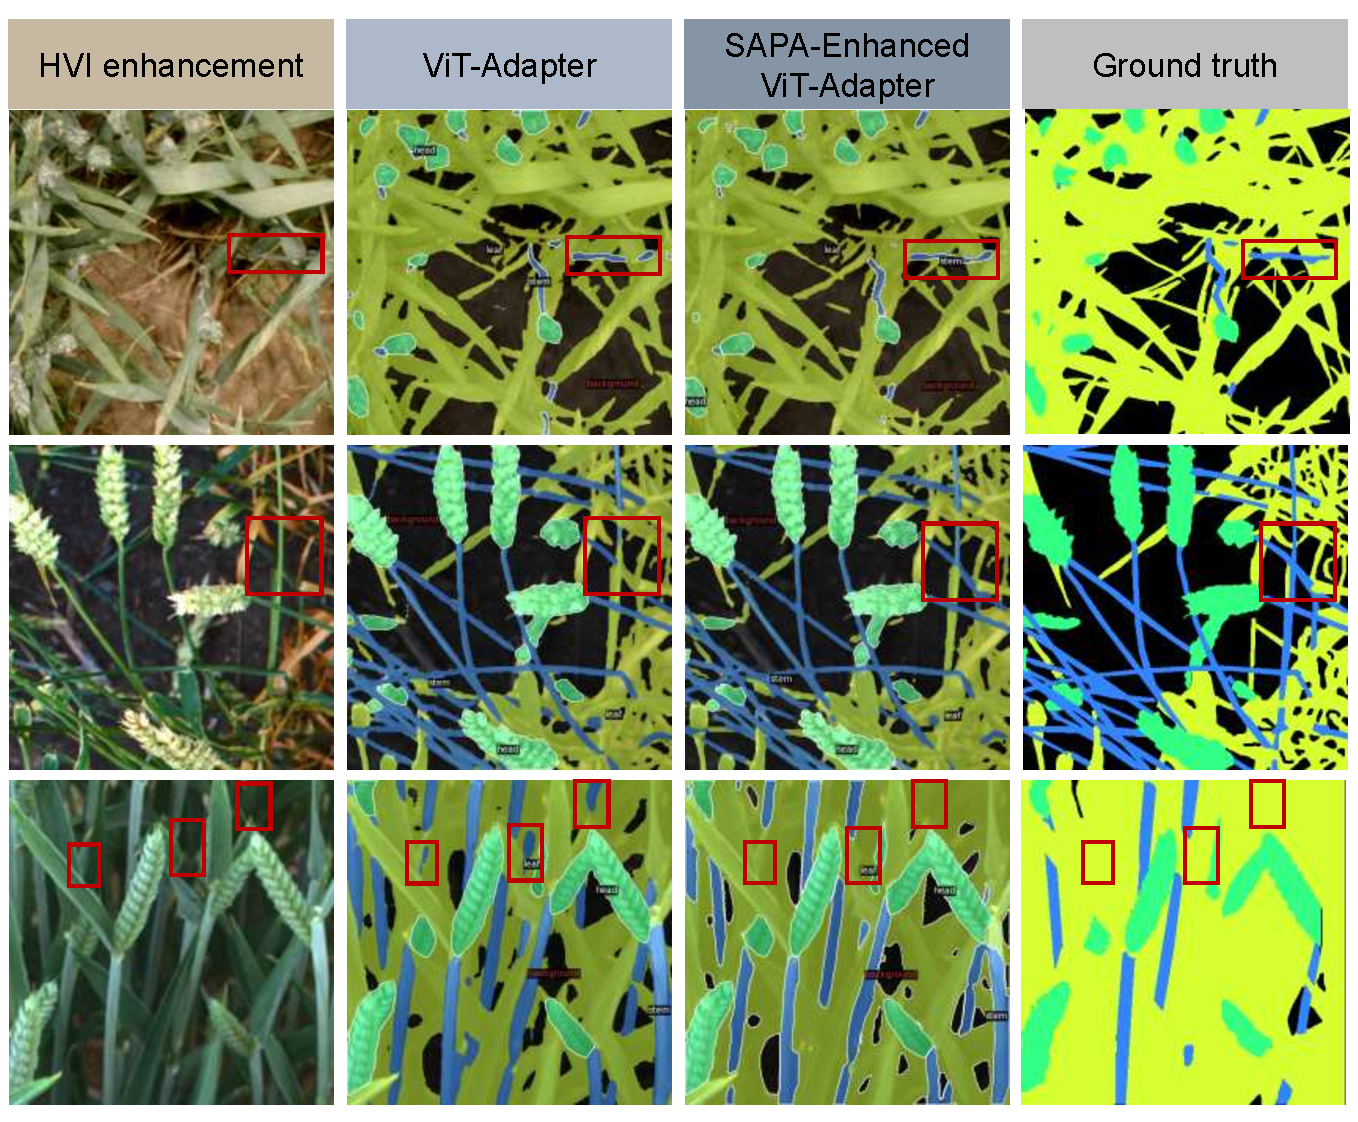
\includegraphics[width=\linewidth]{sapa_baseline.pdf}
    \caption{\textbf{Comparison between the naive ViT-Adapter baseline and SAPA-Enhanced ViT-Adapter}. The red rectangles indicate that SAPA-Enhanced ViT-Adapter is more effective than the vanilla ViT-Adapter in tackling the segmentation of stem structures, with less misclassifications and missing segmentations.}
    \label{fig:sapa_baseline}
\end{figure}

%Specifically, we use the encoder feature $\mathcal{F}_1^{\frac{1}{4}}$ as the guidance to upsample $\mathcal{F}_2^{\frac{1}{8}}$, and the upsampled result is added to $\mathcal{F}_1^{\frac{1}{4}}$. Thus, the model can obtain more accurate per-pixel embeddings and achieve higher performance, compared to using bilinear interpolation upsampling.

%-------------------------------------------------------------------------
\subsection{Guided Distillation with Stem-Aware Sample Selection}
% Considering that the provided unlabeled data may be limited and costly to pretrain a model, we finally choose the second route of semi-supervised learning. 
% Here we present on how we jointly use the labeled and unlabeled training set.
As aforementioned, % to exploit the large amount of unlabeled data provided in the competition, we can use the pipeline 
one can choose two routes, \ie, self-supervised pretraining or semi-supervise learning, to exploit the unlabeled data provided by the competition. We finally choose the second route of semi-supervised learning. The reason is that, although there are over $60,000$ unlabeled images, which is significantly more than the $99$ labeled data, such a data scale % this amount 
may still be insufficient for self-supervised learning to train a robust vision backbone (DINOv2 uses 142M images~\cite{oquab2023dinov2}). Meanwhile, even with a well-pretrained backbone, %  model, 
fine-tuning is still required. % on a small training set, which may risk overfitting. Thus, we finally choose to leverage semi-supervised learning.  
 

Mainstream semi-supervised learning is typically based on the Mean Teacher framework~\cite{tarvainen2017mean}. In % the the distillation-based semi-supervised pipeline
this framework, there is often a Siamese network % often 
with two identical model architectures and parameters, where a teacher model generates soft predictions to guide the training of a student model. The teacher model is updated following the exponential moving average (EMA) with the parameters of the student model. % , ensuring more stable and reliable predictions on unlabeled data. 
Let $\theta_t^{i}$ and $\theta_s^{i}$ denote the weights of the teacher model and the student model at the $i$-th iteration, respectively. % The update founction for 
The teacher model is updated as % can be written as:
\begin{equation}
    \theta_t^{i+1}=\alpha\theta_t^{i} + (1-\alpha)\theta_s^{i+1}\,,
\end{equation}
where $\alpha$ is a damping factor.
For each unlabeled sample, the teacher and student models receive perturbed versions of the same input (e.g., different augmentations), and the student is trained to match the output of the teacher model, % enforcing
encouraging consistency between them. The meta pipeline of mean teacher enables the teacher model to learn from a large amount of unlabeled data and therefore enhances its generalization ability.

In this competition, % When transferring to the semantic segmentation domain, 
we adopt an improved guided distillation framework~\cite{berrada2024guided}. The overview of guided distillation is shown in the stage two of Fig.~\ref{fig:pipeline}. % During the guided distillation stage, 
Most existing distillation-based pipelines train a model on the labeled data as the student. However, this strategy % is not ideal
can be suboptimal in our competition due to the fact that the student model % will be more likely to
may overfit the labeled training data (only $99$ images). To address this, guided distillation introduces a guided burn-in stage, % in the guided distillation pipeline, 
where the student model is allowed to % will 
learn from both labeled and unlabeled data. Before guided distillation, the teacher model is first trained on the labeled data and is used to generate pseudo labels for the student model (the stage one). Then the student model is initialized randomly % from scratch and 
and learned from both labeled and pseudo-labeled data. After the guided burn-in stage, the student model will % be copied to
transfer its weights to the teacher model and perform the standard EMA update. % start to update the teacher model using EMA.

To better adapt this framework to our problem, we further repurpose the idea of importance sampling~\cite{kirillov2020pointrend} by selecting stem-aware samples from the unlabeled data. In particular, considering that the unlabeled data are organized into $9$ domains, we select the top $500$ samples with the most proportion of stem pixels in each domain conditioned on the pseudo-labeled masks, resulting in $4500$ images in total. % We only sample a limited number of points from the high resolution masks using importance sampling. 
The stem-aware sample selection can maximize the presence of the stem class to the model, which somehow mitigates the problem of class imbalance.

The loss functions used follow the Mask2Former~\cite{he2022masked}. Given a wheat image $x_i$ and its ground-truth segmentation mask $y_i=\{(y_i^k,c_i^k)\}_{k\in[1,n]}$ encoded by binary masks $y_i^k$'s and class indices $c_i^k$'s. For each sample, the model predicts $K$ candidate masks $\{(\hat{y}_i^k, \hat{c}_i^k)\}_{1\leq k \leq K }$. After bipartite matching, a matching $(k, m_k)$ is obtained between the predictions and ground truths, where $m_k$ is the index of the predicted mask matched to the $k$-th ground truth mask. The single-sample supervised loss $\mathcal{L}_s^i$ thus can be defined by
\begin{equation}
\begin{aligned}
    \mathcal{L}_s^i=&\frac{1}{n}\sum_{k=1}^{n} \ell_{ce}(\hat{y}_i^{m_k}, y_i^k) +\lambda_{dice} \ell_{dice}(\hat{y}_i^{m_k}, y_i^k) \\
    &+\lambda_{c}\ell_{c}(\hat{y}_i^{m_k}, y_i^k)
\end{aligned}\,,
\end{equation}
where $\ell_{ce}$ is the cross-entropy loss, $\ell_{dice}$ is the dice loss, $\ell_{c}$ is the binary cross-entropy, and $\lambda_{dice}$ and $\lambda_{c}$ are hyperparameters used to control the contribution of different losses. % scaling parameters.
The unsupervised loss $\mathcal{L}_u$ w.r.t. the unlabeled data is identical to the supervised one $\mathcal{L}_s$, except that the ground truth labels are replaced by the pseudo masks generated from the teacher model. By removing the superscript $i$ for $\mathcal{L}_s^i$, the final guided distillation takes the form
\begin{equation}
    \mathcal{L} = \mathcal{L}_s+\lambda_u\mathcal{L}_u\,,
\end{equation}
where % $\mathcal{L}_u$ is the loss of unlabeled data, 
$\lambda_u$ weights the importance of the % is the weight of 
unsupervised loss. Note that, guided distillation only uses $99$ labeled images and the selected $4500$ unlabeled images.

% Since the stem class occupies only a small number of pixels, training may suffer from class imbalance. To address this, we select only unlabeled samples with a high proportion of stem pixels for guided distillation. Specifically, we use the model trained on the labeled training set to infer on the entire pretraining dataset. Based on the predictions, we calculate the pixel proportion of the stem class in each sample, and select the top $500$ samples with the highest stem pixel ratio from each domain. In total, $4,500$ unlabeled samples are selected to use in Stage $2$.

%-------------------------------------------------------------------------
\subsection{Zoom In and Segment Twice}
Small- and fine-object visual perception has % always 
been % important component
long-standing hard cases for % dense prediction
semantic segmentation. % , because they can significantly affect the overall performance. 
In our case, the \texttt{stem} class is identified % seems 
to be the bottleneck due to its not only small-proportion but also fine-structure characteristics. After the stage-two training, we have achieved fairly good performance on the leaderboard, but not competitive enough to secure the first place. Hence, in the rest time of the competition, we start to seek other training-free solutions to improve the performance of the \texttt{stem} class further. % Therefore, we attempt to further improve the segmentation of the stem class during the testing time. 
Inspired by slicing-aided hyper inference~\cite{akyon2022slicing} which has shown strong performance in detecting small objects, we % consider adopting this approach 
adapt this idea to wheat segmentation and develop a test-time scaling strategy called \textit{zoom in and segment twice}. This strategy is initially inspired by an surprising observation that a significant performance improvement can be achieved by simply testing on a zoomed-in version of image. By scaling the image resolution from $512\times512$ to $768\times768$, the performance improves from $0.74$ to $0.76$, which suggests the \texttt{stem} class can benefit from high-resolution inference. 

% HL, use mathmatical symbols next
Formally, given a scaling ratio $\sigma \geq 1$, we define a $\tt{ZoomIn}$ operator such that $I^{\sigma}={\tt{ZoomIn}}(I, \sigma)$, which
zooms in the input image $I$ from its original size $(H,W)$ 
to $I^\sigma$ a larger size $(\sigma H, \sigma W)$. During inference, given a sliding window size $k=(k_h \times k_w)$ with a stride $t=(t_h,t_w)$, where the subscript $h$ and $w$ indicate the height and width components, we further define a $\tt{Slide}$ operator such that 
$
\{I_{i,j}^{\sigma}\}={\tt{Slide}}(I^{\sigma}, k, t) \,,
$
which slides the image $I^{\sigma}$, crop it into sub-window $\{I_{i,j}^{\sigma}\}$, where $\{I_{i,j}^{\sigma}\}=\{I^{\sigma}[i:i+k_h,j:j+k_w]~|~i=0,t_h,...,\sigma H-k_h; j=0,t_w,...,\sigma W-k_w \}$.

For each sliding window, we have the prediction logit for each window $L_{i,j}^s={\tt{Infer}}(I_{i,j}^{\sigma})$, where ${\tt{Infer}}$ means the model inference process. We then apply zero padding to match each logit to the original input resolution and average all the logits. During logit averaging, a count map $C\in \mathbb{R}^{\sigma H\times \sigma W}$ is recorded to % maintained to record 
indicate the number of times each pixel covered by the sliding windows. The final aggregated logit $L^{s}$ is obtained by dividing the summed logits by the count map as
\begin{equation}
     L^{\sigma} 
     =\frac{1}{C}\cdot \sum {\tt Pad}({\tt Infer}({\tt Slide}({\tt ZoomIn}(I,\sigma)), k, t)\,,
\end{equation}
where ${\tt Pad}(\cdot)$ is the zero padding operator. % used to align the model output to the resolution of input image.
% By applying this method, the score in the development phase improved from $0.74$ to $0.76$.

% In addition, we extend the input images to multiple scales.
The `zoom in' strategy can be easily extended to multi-scale scenarios, which implements the `segment twice' idea.
Given a set of multi-scale ratio $S=\{\sigma_0,\sigma_1,...,\sigma_n\}$. For each ratio, we apply the same single-scale inference process above to obtain $L^{\sigma_i}$.
Then, we can simply average the predicted logits across different scales to obtain the final logits
\begin{equation}
    L=\frac{\sum_{\sigma_i \in S}{\tt{DownSample}}(L^{\sigma_i}, \sigma_i)}{|S|}\,,
\end{equation}
where ${\tt{DownSample}(\cdot, \sigma)}$ means downsampling the input with the ratio $\sigma$.
% The scores of different inference scales can be found in Table~\ref{tab:test_time_scale}.


\begin{table}[!t]
    \centering
    \renewcommand{\arraystretch}{1.5}
    \addtolength{\tabcolsep}{-1pt}
    \scalebox{0.86}{
    \begin{tabular}{@{}lcccc@{}}
    \toprule
        \textbf{Method} & \textbf{SAPA} & \textbf{guided distillation} & \textbf{test time scaling} & \textbf{mIoU} \\
    \hline
        baseline & & & & $0.7284$  \\
    \hline
        & \ding{51} & & & 0.7291 \\
        & \ding{51} & \ding{51} &  & 0.7432 \\
        & \ding{51} & \ding{51} & \ding{51} & 0.7704 \\
    \bottomrule
    \end{tabular}}
    \caption{\textbf{Ablation of different stages during the development phase}.}
    \label{tab:ablation}
\end{table}